%%
%% Latex Style File for MECH0020 - AY 2023/2024
%%
%% I. Eames 
%% version 2
%% 26th March 2024
%% Uses vanilla form of latex with no need to additional style files
%%

\documentclass[11pt,twocolumn]{article} 
\usepackage[portuguese]{babel}
\usepackage{fancyhdr}
\usepackage{expl3,xparse,xcoffins,titling,kantlipsum}
\ExplSyntaxOn
\coffin_new:N \l_my_abstract_coffin
\dim_zero_new:N \l_my_width_dim
\keys_define:nn { my / abstract }
  {
    width .code:n = {
      \dim_set:Nn \l_my_width_dim {#1\textwidth}
    }
  }
\NewDocumentCommand \myabstract { O {width=.8} m }{%
  \keys_set:nn { my / abstract } { #1 }
  \SetVerticalCoffin \l_my_abstract_coffin {\l_my_width_dim} {#2}
  \renewcommand\maketitlehookd{%
    \mbox{}\medskip\par
    \centering
    \TypesetCoffin \l_my_abstract_coffin
  }
}
\ExplSyntaxOff
\usepackage[document]{ragged2e}
\usepackage{geometry}
 \geometry{
  a4paper,
  total={170mm,257mm},
  left=17.5mm,
  right=17.5mm,
  bottom=15mm,
  top=15mm
 }

\usepackage{amsmath}
 
 \newcommand\underrel[2]{\mathrel{\mathop{#2}\limits_{#1}}}
 
 \newcommand{\matriz}[1]{\hat#1}
 
 \newcommand{\many}[2]{$#1_1, #1_2, \dots, #1_#2$}
 
 \newcommand{\cmany}[3]{$#1_1 #3 #1_2 #3 \dots #3 #1_#2$}
 
 \newcommand{\mmany}[2]{ #1_1, #1_2, \dots, #1_#2 }
 
 \newcommand{\mcmany}[3]{#1_1 #3 #1_2 #3 \dots #3 #1_#2}
 
 \newcommand{\set}[1]{\{#1\}}
 
 \newcommand{\cjgt}[1]{\overline{#1}}
 \DeclareMathOperator{\diag}{diag}
 \DeclareMathOperator{\sign}{sign}
 \DeclareMathOperator{\ai}{Ai}
 \DeclareMathOperator{\re}{Re}
 \DeclareMathOperator{\im}{Im}
 \DeclareMathOperator{\Df}{D}
 \DeclareMathOperator{\Ee}{E}
 \DeclareMathOperator{\h}{h_1}
 \DeclareMathOperator{\f}{f}
 \DeclareMathOperator{\U}{U}
 \DeclareMathOperator{\W}{W}
 \DeclareMathOperator{\K}{K}
 \DeclareMathOperator{\Hf}{\mathcal{H}}
 \DeclareMathOperator{\Qf}{Q}
 \DeclareMathOperator{\Gl}{\mathcal{L}}
 \DeclareMathOperator{\g}{g}
 \DeclareMathOperator{\V}{V}
 \newcommand{\iu}{\mathrm{i}\mkern1mu}
 \DeclareMathOperator{\ee}{\textrm e}
 \DeclareMathOperator{\supp}{supp}
 \renewcommand{\Re}{\mathop{\textrm Re}}
 \newcommand{\res}{\mathop{\textrm Res}}
 \renewcommand{\Im}{\mathop{\textrm Im}}
 \newcommand{\N}{\mathbb{N}}
 \newcommand{\C}{\mathbb{C}}
 \newcommand{\R}{\mathbb{R}}
 \newcommand{\Z}{\mathbb{Z}}
 \newcommand{\D}{\mathbb{D}}
 \newcommand{\Q}{\mathbb{Q}}
 \newcommand{\J}{J} %Jacobiano
 \newcommand{\Id}{\mathbb{1}}
 \newcommand{\p}{p} %medida
 \newcommand{\E}{\mathbb{E}}
 \newcommand{\Se}{\mathbb{S}}
 \newcommand{\He}{\mathbb{H}}
 \newcommand{\boh}{\mathit{o}}
 \newcommand{\Boh}{\mathcal{O}}
 \newcommand{\bbp}{\bm K_{\mathrm{BBP}}}
 \newcommand{\ii}{\mathrm{i}}
\usepackage{amsfonts}
 \usepackage{amssymb}
% \documentclass{gji}
\usepackage{timet,color}
\usepackage{nomencl}
\setlength{\nomitemsep}{-\parsep}
\usepackage{graphicx}
\usepackage[urlcolor=blue,citecolor=black,linkcolor=black]{hyperref}
\usepackage{times}
\usepackage{multicol}
\usepackage{physics}
\usepackage{bbm}


% MATH DECLARATIONS
\newtheorem{lemma}{Lema}[section]
\newtheorem{thm}[lemma]{Teorema}
\newtheorem{claim}[lemma]{Afirmação}
\newtheorem{cor}[lemma]{Corolário}
\newtheorem{definition}[lemma]{Definição}
\newtheorem{conjecture}[lemma]{Conjectura}
\newtheorem{prop}[lemma]{Proposição}
\newtheorem{assumption}[lemma]{Assumpção}
\numberwithin{equation}{section} %numeracao dentro de secoes

% PROOF ENV
\makeatletter
\newenvironment{proof}[1][Demonstração]{\par
	\pushQED{\qed}%
	\normalfont \topsep6\p@\@plus6\p@\relax
	\trivlist
	\item\relax
	{\itshape
		#1\@addpunct{.}}\hspace\labelsep\ignorespaces
}{%
	\popQED\endtrivlist\@endpefalse
}
\makeatother



\makenomenclature
\begin{document}

\title{\bf \Huge Matrizes Aleatórias e Simulação de Gases de Coulomb}
\author{{\bf \Large João Victor Alcantara Pimenta$^1$, Guilherme Silva$^2$}\\
  $^1$ Instituto de Física de São Carlos, IFSC - USP \\
  $^2$ Instituto de Ciências Matemáticas e Computação, ICMC - USP
  }
\date{Abril, 2024}


\let\leqslant=\leq

\label{firstpage}


%%
%% This format for begin abstract is a reclaration of a macro to 
%% create single columne for abstract
%%
\justifying
\myabstract[width=0.9]{
O estudo do espectro de matrizes aleatórias demonstra aplicabilidade em uma gama diversa de áreas da física, matemática à computação e engenharia. Estudamos os principais ensembles da Teoria de Matrizes Aleatórias e suas medidas de equilíbrio, e, utilizando da analogia de Gases de Coulomb, realizamos simulações que nos permitem calcular médias de funções de interesse. Discute-se quais métodos são importantes para a simulação do problema de gases de coulomb e quais suas limitações, além das impostas pela escalabilidade e singularidades do problema. Mostramos que o método de \textit{Langevin Monte Carlo} tem boa performance, possibilitando a réplica de medidas para modelos bem descritos em uma dimensão. Discute-se como esse resultado é importante e quais suas possíveis extensões.
\noindent
}


\maketitle

%%
%% This creates a header title for MECH0020_AY2023-24
%%
\pagestyle{fancy}
\fancyhead[L]{SENIC SBM - 2024}
%%
%% This creates the nomenclature list - dont forget to tag the 
%% definitions for new symbols as you go through
%%

\printnomenclature

\section{Introdução}

De acordo com a mecânica quântica, níveis de energia de uma sistema são descritos pelos autovalores de seu operador hermitiano associado, o hamiltoniano $\Hf$. Em situações mais complexas, $\Hf$ não é completamente descrito pela teoria ou é complicado. Por isto, somado à necessidade do cálculo explícito de grandezas, considera-se usualmente truncamentos do espaço de Hilbert onde opera $\Hf$, representado agora por matrizes de dimensão finita. Caracterizar o sistema físico é resolver o problema de autovalores $\Hf \Psi_i = E_i \Psi_i$. Wigner, em seu estudo de núcleos atômicos, foi um dos primeiros a sugerir uma solução alternativa, uma mecânica estatística para o problema de autovalores. Tal teoria descreveria o perfil da estrutura energética nucleica ao invés de detalhar seus níveis, impondo perguntas estocásticas ao invés de determinísticas, que comumente seriam impossíveis de responder. Buscava-se, em algum sentido, uma universalidade, uma resposta que fosse, dada complexidade o suficiente, independente de $\Hf$. A teoria foi prontamente seguida por, dentre outros, Porter e Rosenzweig , que procederam a validar com dados experimentais as ideias postuladas e por Gaudin, Mehta, e Dyson, que avançaram na descrição, dentre outros, dos importantes ensembles gaussianos. Esse desenvolvimento e seus desdobramentos veio a ser o que chamamos hoje de Teoria de Matrizes Aleatórias (RMT, \textit{Random Matrix Theory}). Hoje, suas aplicações são extensas em campos de alta complexidade ou com descrição matricial, principalmente quando há estrutura, como matrizes de correlação ou operadores físicos.

Seja $\Se$ um conjunto tal como $\R, \C, \He $ (Reais, Complexos e Quaterniônicos). Considere uma matriz $\matriz{M} \in \mathcal{M}_{\Se}(N)$ espaço de matrizes $N \cross N$, ou seja, de $N^2$ entradas, sejam elas reais, complexas ou quaterniônicas. Se tomamos o elemento de matriz $M_{i,j}$ $\forall i, j \in \Z$, com $1 \leq i, j \leq N$, como variável aleatória de distribuição arbitrária, podemos expressar a densidade de probabilidade conjunta (jpdf, \textit{joint probability density function}) como $$\p(\hat{M}) \dd M = \p(M_{1,1}, \dots, M_{N,N}) \prod_{i,j=1}^{N} \dd M_{i,j}.$$

Não lidaremos, contudo, com uma classe tão ampla de matrizes. Considere a decomposição $\matriz{M} = \matriz{O} \matriz{D} \matriz{O}^{-1}$, onde $\matriz{D} = \diag(\mmany{\lambda}{N})$. Estamos especialmente interessados no caso onde $\matriz{O} \in V_N(\Se^N)$, espaço denominado variedade de Stiefel. Isso implica que $ \matriz{O} \matriz{O}^* = \mathbbm{1}$. Tomamos $\matriz{O}$ matriz ortogonal, unitária ou simplética, a depender de $\Se$, o que resulta em autovalores $\lambda \in \R$. Isto pode ser motivado fisicamente sabendo que, para sistemas quânticos invariantes reversíveis, o Hamiltoniano é matriz real simétrica; na presença de campo magnético, o Hamiltoniano é matriz complexa hermitiana; na presença de acoplamento spin-órbita, o Hamiltoniano é simplético \cite[Capítulo~2]{RMT-firstcourse-Potters}.

Para o subespaço tomado vale que $\cjgt{M_{i,j}} = M_{j, i}$. Este vínculo reflete na dimensão do subespaço escolhido, com valor dependente de $\Se$. A transformação tomada tem ainda Jacobiano $\J(\matriz{M} \rightarrow \{ \vec{\lambda}, \matriz{O} \} )$ que pode ser calculado explicitamente. Ressalta-se que estamos interessados em distribuições de autovalores. Para calcular $\p(\mmany{\lambda}{N})$ devemos integrar a jpdf sobre o subespaço $V_N(\Se^N)$. Isso nem sempre é fácil ou possível. Para garantir a integrabilidade, tomaremos \textit{ensembles} de matrizes aleatórias onde o jpdf de suas entradas $\p(\mmany{\lambda}{N}, \matriz{O})$ pode ser escrito exclusivamente como função dos autovalores $$\p \left( M_{1,1}(\vec{\lambda}), \cdots, M_{N,N}(\vec{\lambda}) | \J(\matriz{M} \rightarrow \{ \vec{\lambda} \} ) \right).$$

Ensembles com esta propriedade são denominados invariantes por rotação. Esta escolha implica que quaisquer duas matrizes $\matriz{M}, \matriz{M'~}$ que satisfaçam a relação de equivalência $\matriz{M} = \matriz{U} \matriz{M'} \matriz{U}^{-1}$ tem mesma probabilidade. Nesta relação, $\matriz{U}$ é simétrica, hermitiana ou simplética respectivamente quando $\Se = \R,\C,\He $. Considere o teorema \cite[Capítulo~3]{AlanThesis}.
\begin{thm}
	Tome $\matriz{M} \in M_{\R}(N),  M_{\C}(N),  M_{\He}(N)$ simétrica, hermitiana ou autodual, respectivamente. Se  $\matriz{M}$ tem jpdf da forma $\phi(\matriz{M})$, invariante sobre transformações de similaridade ortogonal, a jpdf dos $N$ autovalores ordenados de $\matriz{M}$, $\mcmany{\lambda}{N}{\geq}$, é $$ C_{N}^{(\beta)} \phi(\matriz{D}) \prod_{i < j} (\lambda_i - \lambda_j)^{\beta}$$ onde $C_{N}^{\beta}$ é constante e $\beta = 1, 2, 4$ corresponde respectivamente à $\matriz{M} \in M_{\R}(N),  M_{\C}(N),  M_{\He}(N)$. 
	\label{Teorema: Invariante}
\end{thm}

Logo, desde que tomemos um ensemble de matrizes aleatórias com a jpdf das entradas apropriado, podemos reescrever a distribuição em função dos autovalores com \ref{Teorema: Invariante}. Vale ainda observar que, pelo Lema de Weyl, uma jpdf invariante pode ser expressa totalmente por $\p(\matriz{M})= \phi \left(\Tr(F(M)) \right)$ com $F$ função polinomial, ou ainda
\begin{equation}
	\p_{ord}(\vec{\lambda}) = C_{N}^{\beta} \phi{\left( \sum_i^N F(\lambda_i) \right)} \prod_{i < j} (\lambda_i - \lambda_j)^{\beta}.
	\label{Equation: p-ord}
\end{equation}

Dentre os muitos ensembles em RMT, os Gaussianos são notórios. São eles o \textit{Gaussian Orthogonal Ensemble (GOE)} ($\beta=1$), \textit{Gaussian Unitary Ensemble (GUE)} ($\beta=2$) e \textit{Gaussian Sympletic Ensemble (GSE)} ($\beta=4$). Notemos primeiramente que o nome é relacionado à escolha de $\Se$. Mais explicitamente, o nome é dado em relação à se $\matriz{O}$, tal que $\matriz{M} = \matriz{O}\matriz{D}\matriz{O}^*$, é ortogonal, unitário ou simplético. É natural então pensar nos ensembles \textit{GOE}, \textit{GUE} e \textit{GSE} como matrizes $\matriz{M} \in \mathcal{M}_{\Se}(N)$ onde 
$$
\mathcal{M}_{\Se}(N) \ni M_{i,j} \sim
\begin{cases}
	\mathcal{N}_{\Se}(0,1/2) &  \ \text{para} \ i \neq j,\\
	\mathcal{N}_{\Se}(0,1) & \ \text{para} \ i = j.
\end{cases}
$$

Os três ensembles gaussianos compartilham de uma propriedade exclusiva - são os únicos ensembles com entradas independentes e, simultaneamente, jpdf rotacionalmente invariante. Podemos deduzir, para $\beta = 1,2,4$ que
\begin{equation}
	\p(\vec{\lambda}) = \frac{1}{Z_{N, \beta}} \ee^{-\beta_N \mathcal{H}_N(\vec{\lambda})},
	\label{Equation: medida Gaussian}
\end{equation}
onde $Z_{N, \beta}$ é função de partição canônica para autovalores desordenados\footnote{Usa-se do fator de contagem de Boltzmann para escrever $ Z_{N, \beta} = N! Z_{N, \beta}^{(ord)}$.}, normalizante da expressão \ref{Equation: medida Gaussian}. O fator $\beta_N = \beta N^2$ é pensado como a temperatura inversa. Definimos ainda o Hamiltoniano $$\mathcal{H}_N(\vec{\lambda}) = \frac{1}{N}\sum_{i = 1}^{N} \frac{\lambda_i^2}{2} + \frac{1}{N^2} \sum_{i < j} \log{\frac{1}{|\lambda_i - \lambda_j|}}$$ com  $\lambda_i \mapsto \lambda_i \sqrt{\beta N}$.

\section{Gases de Coulomb}

Para os ensembles que chamamos invariantes, a densidade de autovalores guarda uma importante analogia, a de Gases de Coulomb. Pensando os $N$ autovalores das matrizes como partículas de um gás com o devido núcleo de interação e potencial externo, podemos usar de noções físicas para intuir seu comportamento. Usando das estabelecidas leis termodinâmicas é possível ainda derivar, por exemplo, as densidades de autovalores no limite termodinâmico ($N \rightarrow \infty$). Generalizando o potencial aplicado podemos ainda recuperar um ensemble de matrizes que pode não estar diretamente disponível. Usar de simulações de gases para extrair medidas tem algumas dificuldades. Nem sempre uma solução analítica é possível para as equações diferencias que descrevem sua dinâmica, que deve ser ergótica. Por isso, recorre-se à simulações numéricas que podem também se mostrar delicadas de tratar. A dinâmica tem alta complexidade temporal pela quantidade de interações entre partículas e as singularidades dificultam a invariância do hamiltoniano na simulação. Ainda assim, essa abordagem permite explorar ensembles exóticos em RMT e será discutida nesse trabalho.

% Sabemos então, que a partir dessa função podemos retirar importantes propriedades estatísticas (macroscópicas) do sistema de autovalores dos ensembles Gaussianos.

Sob as devidas condições, o gás de coulomb $\p_N$ \cite{ChafaCoulombMeasure} é a medida de probabilidade de Boltzmann-Gibbs dada em $(R^d)^N$ por 
\begin{equation}
	\dd \p_N(\vec{x}) = \frac{e^{-\beta N^2 \Hf_N(\vec{x})}}{Z_{N,\beta}} \dd \vec{x},
	\label{Equação: Medida Gas de Coulomb}
\end{equation}
onde $$\Hf_N(\vec{x}) = \frac{1}{N} \sum_{i = 1}^{N} \V(x) + \frac{1}{2N^2} \sum_{i \neq j} \g(x_i - x_j)$$ é usualmente chamado hamiltoniano ou energia do sistema. A medida $\p_N$ modela um gás de partículas indistinguíveis com carga nas posições $\mmany{x}{N} \in \Se$ de dimensão $d$ em $\R^n$ \textit{ambient space}. As partículas estão sujeitas a um potencial externo $\V \colon \Se \mapsto \R$ e interagem por $\g \colon \Se \mapsto (-\infty, \infty]$. A temperatura inversa é $\beta N^2$. Assumiremos, para que valha a definição \ref{Equação: Medida Gas de Coulomb}, que $V, \ \g \ \text{e} \ \beta$ são tais que a constante de normalização (função partição) $Z_{N, \beta} < \infty \ \forall \ N$\footnote{Note que $\p_N$ é um modelo de interações estáticas e não há campos magnéticos considerados.}. Tome $\R^n$ com $n \geq 2$, sabemos que, para $x \neq 0$ o núcleo de interação coulombiana (função de Green) vale $$
g(\vec{x}) =
\begin{cases}
	\log \frac{1}{|\vec{x}|} \ \ \text{se} \ n = 2,\\
	\frac{1}{|x|^{n-2}} \ \ \text{se} \ n \geq 3.
\end{cases}
$$ onde $g$ é solução da equação de Poisson.

Se lembramos da expressão \ref{Equation: medida Gaussian}, perceberemos que, para o devido $\V(x)$, podemos tomar $d=1$ e $n = 2$ para recuperar a medida dos ensembles gaussianos 
\begin{equation}
	\p_N(\vec{x}) = \frac{e^{-\beta_N \Hf_N(\vec{x})}}{Z_{N,\beta}},
	\label{Equation: Medida Log V}
\end{equation}
\begin{equation}
	\Hf_N(\vec{x}) = \frac{1}{N} \sum_{i = 1}^{N} \V(x_i) + \frac{1}{N^2} \sum_{i < j} \log{\frac{1}{|x_i - x_j|}}.
\end{equation}
Estamos tratando de partículas no plano confinadas à uma reta. Para algum potencial arbitrário, além da devida escolha de $n$ e $d$, cairemos em outros ensembles de matrizes.

O conjunto de pontos no espaço de fase ou ainda, os microestados, determinam um \textit{ensemble estatístico}. De mesma forma, um conjunto de matrizes determina um ensemble em RMT. Podemos relacionar o conjunto de microestados dos autovalores $\{\vec{\lambda}\}$ com as configurações do sistema de $N$ partículas descrito pelos Gases de Coulomb. Notando que tratamos do ensemble canônico, um argumento termodinâmico nos indica então que devemos minimizar a energia livre $$E^V_{N,\beta} = \log{Z_{N, \beta}}.$$

Consideraremos $\V$ sob condições tais que seja denominado um potencial admissível \cite{ChafaCoulombMeasure}. Com isso, se $\mu_{V}(\vec{\lambda})$ é medida de probabilidade no espaço das possíveis configurações de autovalores, $Z_{N, \beta}$ será finita e existirá $\mu_{V}^* = \arg \inf {\mathcal{H}_N(\vec{\lambda})}$ medida de equilíbrio única no limite termodinâmico $N \rightarrow \infty$. Para determinar a medida de equilíbrio de \ref{Equation: Medida Log V} \cite{RMT-firstcourse-Potters}, queremos satisfazer o sistema de equações
\begin{equation}
	\frac{\partial \mathcal{H}}{\partial \lambda_i} = 0 \ \implies \ \V'(\lambda_i) = \frac{1}{N} \sum_{1 = j \neq i}^{N} \frac{1}{\lambda_i - \lambda_j} \ \ \forall i.
	\label{Equação: Sistema minimizante}
\end{equation} 
Usaremos o denominado \textit{resolvent}. Considere a função complexa $$G_N(z) = \frac{1}{N} \Tr{\left(z \mathbbm{1} - \matriz{M}\right)^{-1}} = \frac{1}{N} \sum_{i=1}^{N} \frac{1}{z - \lambda_i},$$ onde $\matriz{M}$ é matriz aleatória com autovalores $\{\mmany{\lambda}{N}\}$. Note que $G_N(z)$ é uma função complexa aleatória com polos em $\lambda_i$. Não trivialmente, podemos reescrever \ref{Equação: Sistema minimizante} como $$\V'(z) G_N(z) - \Pi_N(z) = \frac{G_N^2(z)}{2} + \frac{G'_N(z)}{2N},$$ onde $\Pi_N(z) = \frac{1}{N} \sum_{i = 1}^{N} \frac{\V'(z) - \V'(\lambda_i)}{z - \lambda_i}$ é um polinômio de grau $\deg{\V'(z)} - 1 = k - 1$. Poderíamos tentar resolver explicitamente essa formula para qualquer $N$, isso é possível em alguns casos. Contudo, em geral, estaremos interessados na assintótica $N \to \infty$ de $G_N(z)$, nesse limite temos a transformada de Stieltjes $S^{\mu_V}(z)$
\begin{equation}
	\int \frac{\mu^*_V(\lambda)}{z - \lambda} \dd \lambda= \V'(z) \pm \sqrt{\V'(z)^2 - 2 \Pi_{\infty}(z) }.
	\label{Equation: Resolvent}
\end{equation}
com $\Pi_{\infty}(z) = \int \frac{\V'(z) - \V'(\lambda)}{z - \lambda} \mu^*_V(\lambda) d\lambda$. Como consequência da fórmula de Sokhotski-Plemeji, é enunciado o resultado 
\begin{equation}
	\begin{split}
		\mu^{*}_{V}(x) 
		&= \frac{1}{2\pi \ii} \left( S^{\mu_V}_{+} -  S^{\mu_V}_{-}\right) \\
		&= \frac{1}{\pi} \lim_{\epsilon \to 0^+} \Im{S^{\mu_V}_{+}(x + \ii\epsilon)}.
	\end{split}
	\label{Equation: p(lambda)}
\end{equation}
%Considere ainda um potencial $\V(x)$ convexo. Neste caso, tomamos naturalmente $\mu^*_V(x)$ não nula apenas em um intervalo $(\lambda_{-}, \lambda_{+})$. Sabemos que o comportamento não analítico surge da raiz quadrada, tal que se definirmos $\Df(z) := \V'(z)^2 - 2 \Pi_{\infty}(z)$ polinômio de grau $2k$, $\{\lambda_{-}, \lambda_{+}\}$ são suas raízes e o polinômio tem valor negativo em algum intervalo. Equivalentemente $D(z) = (z-\lambda_{-})(z - \lambda_{+}) \Qf^2(z),$ onde $\Qf(z)$ é polinômio de grau $k-1$. Com essas definições podemos escrever que, por \ref{Equation: p(lambda)},
%\begin{equation}
%	\mu^*_V(x) =\frac{\Qf(x)}{\pi} \sqrt{(\lambda_{+} - x)(x - \lambda_{-})}, \ \ \text{para} \ \  \lambda_{-} \leq x \leq \lambda_{+}.
%\end{equation}
Restaria, para cada potencial, balancear o sistema de $k+2$ equações dada por
\[
\left( S^{\mu_{V}} - \V' \right)^2 = \left( V' \right)^2 - 2 \Pi_{\infty}
\]

\section{Simulações}
A medida $\mu$ de Boltzmann-Gibbs descreve o denominado ensemble canônico. Médias sobre suas configurações, microestados, são usadas para inferir informações macroscópicas do sistema. Sistemas dinâmicos que amostrem da medida $\mu$ são denominados termostatos e são notoriamente difíceis de se construir ergoticamente com processos dinâmicos determinísticos, portanto, uma teoria de equações diferenciais estocásticas foi desenvolvida. Usualmente, para o ensemble canônico, uma escolha natural de processo é a denominada \textit{Langevin Dynamics} \cite[Capítulo~6]{leimmolecular}, especialmente sua versão cinética. Muitas vezes as equações usadas não são diretamente integráveis e, por isso, se recorre a métodos numéricos. O caso cinético pode ser separado em duas dinâmicas. Para a integração da primeira, chamada Hamiltoniana, utilizamos o esquema de Verlet \cite{Verlet}. Para a segunda parte, denominada flutuação-dissipação, resolve-se analiticamente por se tratar de processo de Ornstein-Uhlenbeck de variância explícita. Apesar das qualidades dos métodos citados, a discretização pode introduzir instabilidade numérica e, para amenizar seus efeitos, introduz-se um passo de Metropolis \cite[Apêndice~C]{leimmolecular}. As escolhas supracitadas são descritas em \cite{Chafa2018} e é denominada \textit{Langevin Monte Carlo}. Simular gases de coulomb é especialmente interessante quando não há modelos de matrizes conhecidos, disponíveis ou simples para o $\Hf$ definido. Podemos, com a simulação de tais gases, calcular a média da função densidade das partículas, ou autovalores.

 Consideraremos nossas $N$ partículas em um subespaço $S$ de dimensão $d$ em $\mathbb{R}^n$ de forma que nosso espaço de fase $\Omega$ será de dimensão $Nd$. O campo externo é $V : S \mapsto \mathbb{R}$ e o núcleo de interação entre as partículas é função $\W : S \mapsto (-\infty, \infty]$. Sob essas condições, temos o algoritmo, descrito em \cite{Chafa2018}, completo. Dada uma condição inicial $(q_k, p_k)$, para cada $k\geq0$, realizamos os seguintes passos
\begin{enumerate}
	\item Baseado no processo de Ornstein-Uhlenbeck, atualize a $\tilde{\p}_k$ com
	\begin{equation}
		\tilde{p}_k = \eta p_k + \sqrt{\frac{1-\eta^2}{\beta_N}} G_k, \ \eta = \ee^{-\gamma_N \alpha_N \Delta t};
		\label{Equation: Alg Mehler}
	\end{equation}
	\item Utilizando do esquema de Verlet, calcule os termos
	\begin{equation}
		\begin{cases}
			\tilde{p}_{k+\frac{1}{2}} = \tilde{p}_k - \nabla H_N(q_k) \alpha_N \frac{\Delta t}{2}, \\
			\tilde{q}_{k+1} = q_k + \tilde{p}_{k + \frac{1}{2}} \alpha_N \Delta t, \\
			\tilde{p}_{k+1} = \tilde{p}_{k+\frac{1}{2}} - \nabla H_N(q_{k+1}) \alpha_N \frac{\Delta t}{2};
			\label{Equation: Alg Verlet}
		\end{cases}
	\end{equation}
	\item Pela definição do passo de metropolis, defina a probabilidade $P_k$
	\begin{equation}
		1 \wedge \ee^{ -\beta \left( H_N(\tilde{q}_{k+1}) + \frac{\tilde{p}^2_{k+1}}{2} - H_N(q_k) - \frac{\tilde{p}^2_k}{2} \right) };
		\label{Equação: Alg Pk}
	\end{equation}
	\item Defina, a partir do cálculo anterior, 
	\begin{equation}
		(q_{k+1}, p_{k+1}) = 
		\begin{cases}
			(\tilde{q}_{k+1}, \tilde{p}_{k+1}) \ \text{c/ prob.} \ P_k, \\
			(q_k, -\tilde{p}_{k}) \ \text{c/ prob.} \ 1-P_k; \\
		\end{cases}
		\label{Equation: Alg Metro}
	\end{equation}
\end{enumerate}

O ajuste de variáveis é notoriamente um dos aspectos complicados do algoritmo implementado. Precisamos de uma holística par ajustar $\Delta t, \alpha_N \ \text{e} \ \gamma_N$. No escopo do nosso programa, $\Delta t$ e $\alpha_N$ desempenham o mesmo papel e, por isso, tomaremos $\alpha_N = 1$ e decidiremos sobre o valor de $\Delta t$. Seguindo a recomendação de \cite[Capítulo~5]{handbookmontecarlo}, tomaremos $\Delta t = \Delta\tilde{t} + X$, onde $X$ é variável aleatória de média $0$ e variância $\sigma^2$ pequena. Essa escolha ajuda a acelerar a convergência em casos exóticos, que queremos evitar. Lembramos ainda que $\Delta \tilde{t}$ é melhor quando é da ordem de $N^{-\frac{1}{4}}$, isto é, é pequeno o suficiente para manter a razão de aceite do passo de Metropolis alta e grande o suficiente para não desacelerar a convergência do algoritmo. Já $\gamma_N$ definirá o quanto substituiremos o momento anterior das partículas e o quanto utilizaremos do passo aleatório. Aqui, sabemos apenas que tornar $\eta$ próximo demais de $0$, ou de $1$ para todos efeitos, desacelera intensamente a convergência. Faremos, em geral, com que $\gamma_N \alpha_N \Delta t \approx 0.5$.

\section{Resultados e Discussão}

Podemos validar a execução do programa e qualidade da medida gerada utilizando de potenciais bem descritos na literatura. A família de ensembles gaussianos são modelos que mostramos ser bem representados como matrizes. Tomar a medida dos ensembles gaussianos é o equivalente na simulação descrita a tomar $d = 1, \ \  n = 2, \ \ \beta_N = \beta N^2$ para $\beta = 1,2,4$ e 
\begin{equation}
	\V(x)=\frac{|x|^2}{2}, \ \ W(x) = g(x) = \log{|x|}.
	\label{Equation: Parametros Gaussian}
\end{equation}
O resultado da simulação para \ref{Equation: Parametros Gaussian} está na Figura \ref{Figura: Gaussian}. Apresentamos ainda na coluna da esquerda os resultados, para $N=10$, da densidade gerada pela simulação equivalente com matrizes para os três modelos ($\beta = 1,2,4$). Na coluna central, representa-se uma comparação com o Semi-Círculo de Wigner, configuração de equilíbrio para os três modelos quando $N$ é grande o suficiente. Note que os valores foram escalados por $\sqrt{2 \beta}$ para melhor visualização. Finalmente, na coluna da direita apresentamos a distribuição do maior autovalor. Um resultado importante  \cite{Tracy} enuncia que existem $z_{N}^{(\beta)}$ e $s_N^{(\beta)}$ tais que $$\lim_{N \to \infty} \mathbb{P}_{\beta,N,V} \left( \frac{\lambda_{max} - z_{N}^{(\beta)}}{s_N^{(\beta)}} \leq x \right) = F_{\beta}(x),$$ onde $F_{\beta}(x)$ é a densidade acumulada de Tracy-Widow. Mostraremos a concordância desse resultado com a simulação na coluna da direita.

\begin{figure}[ht!]
	\centering
	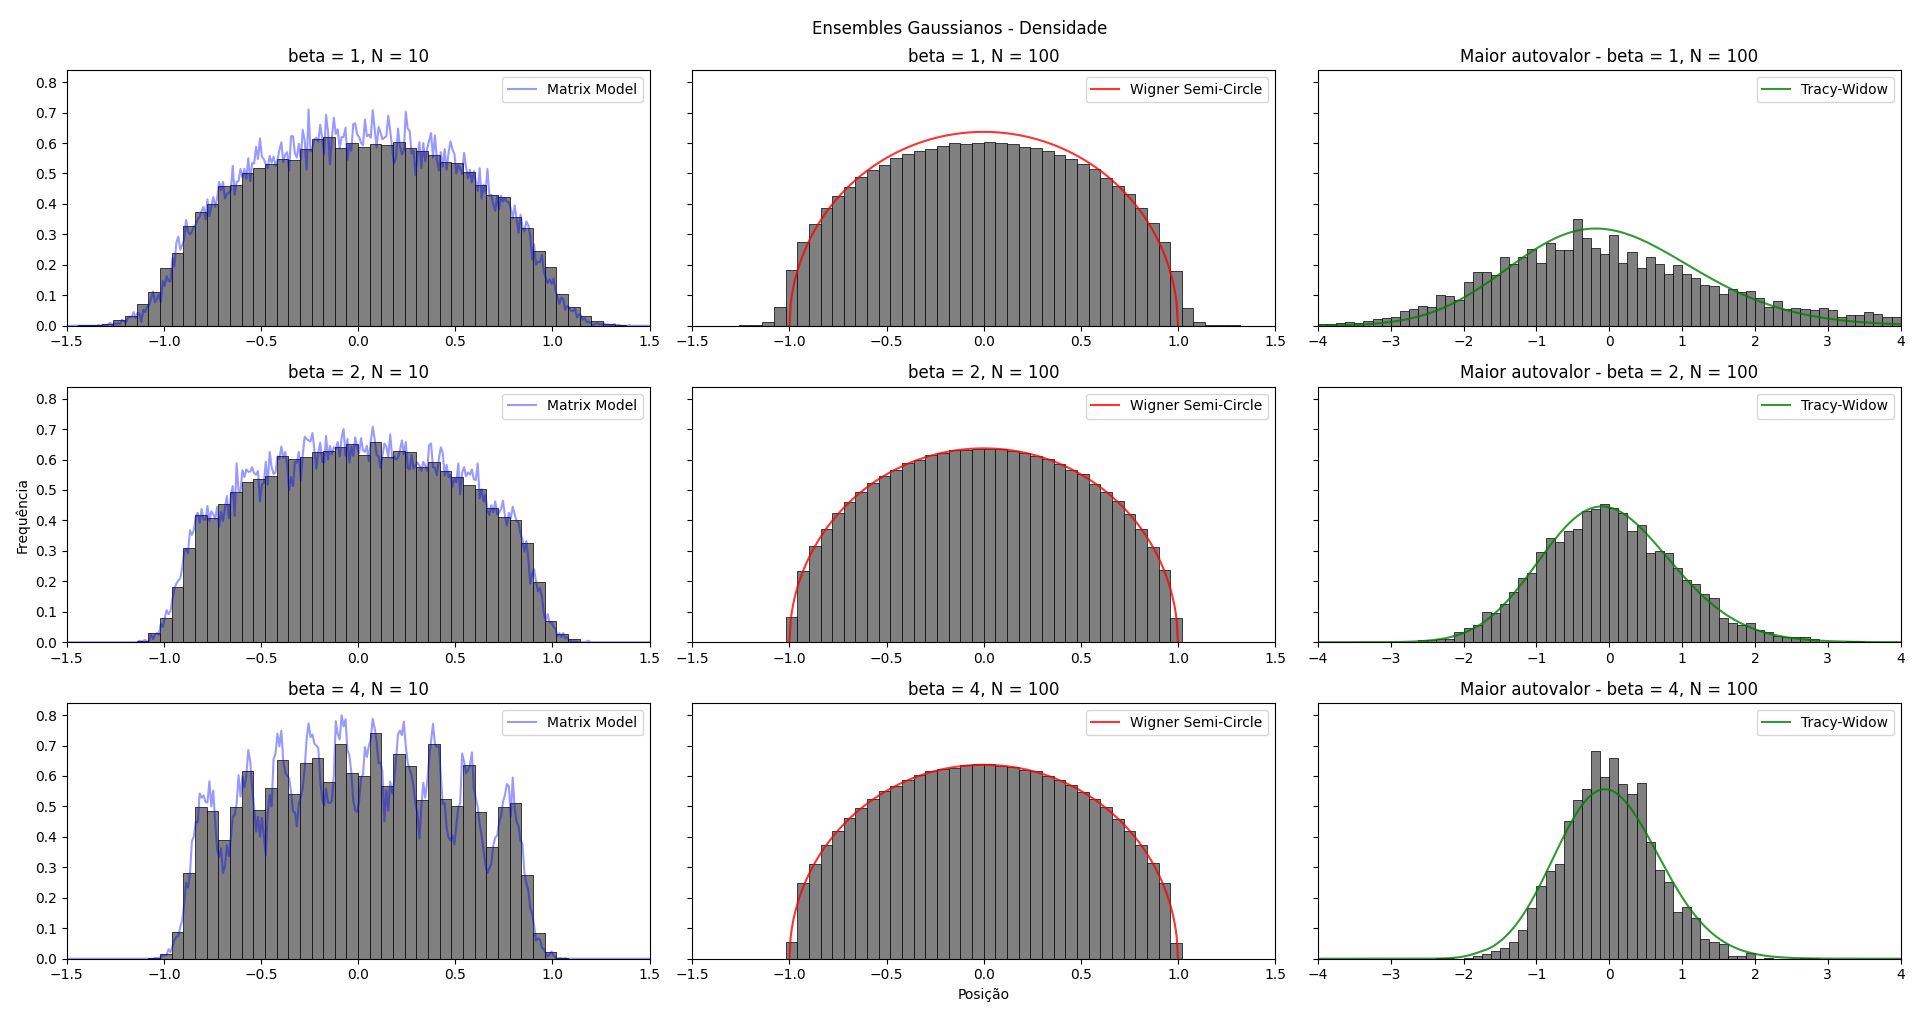
\includegraphics[width=0.45\textwidth]{figures/validationGaussianTracy.png}
	\caption{Densidade para ensembles gaussianos, \ref{Equation: Parametros Gaussian}. Tomou-se $\Delta t = 0.3$ e $nsteps = 5\cdot10^6$ passos, registrando a cada $1000$ iterações a partir de $nsteps/5$. À esquerda da figura, em azul, a densidade da amostragem de $4\cdot10^3$ matrizes do ensemble. No centro, o Semi-Círculo de Wigner, medida de equilíbrio. Na direita, apresenta-se a densidade de $\lambda_{max}$ normalizado e sua mediada esperada.}
	\label{Figura: Gaussian}
\end{figure}

Indo além dos modelos gaussianos podemos retomar as descrições dos potenciais mônico e quártico. Respectivamente, estes modelos equivalem a tomar na simulação os parâmetros $d = 1, \ \  n = 2, \ \ \beta_N = \beta N^2$ para $\beta = 2$ com
\begin{equation}
	\V(x)= t |x|^{2m}, \ \ W(x) = g(x) = \log{|x|}.
	\label{Equation: Parametros Monico}
\end{equation}
e $d = 1, \ \  n = 2, \ \ \beta_N = \beta N^2$ para $\beta = 2$ com
\begin{equation}
\V(x)=\frac{|x|^4}{4} + t \frac{|x|^2}{2}, \ \ W(x) = g(x) = \log{|x|}.
	\label{Equation: Parametros Quartico}
\end{equation}
O caso mônico se reduz ao gaussiano se $m=1$. Os resultados para ambos os potenciais estão explicitados na Figura \ref{Figura: Quartic Monic} para alguns parâmetros interessantes de $t$ e $m$.
\begin{figure}[ht!]
	\centering
	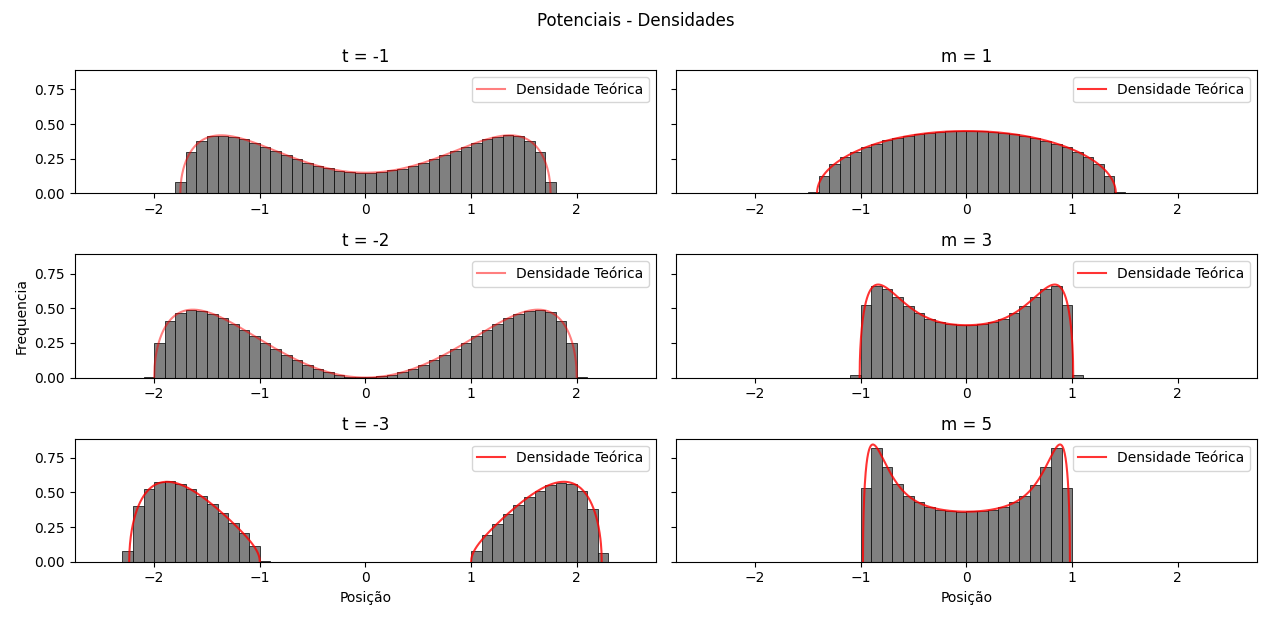
\includegraphics[width=0.45\textwidth]{figures/validationQuarticMonic-alt.png}
	\caption{Potencial Quártico \ref{Equation: Parametros Quartico} e Mônico \ref{Equation: Parametros Monico}, respectivamente à esquerda e direita. Tomou-se $\Delta t = 0.1$, $N=100$, e $nsteps = 5\cdot10^6$ passos. Registra-se a cada $1000$ iterações a partir de $nsteps/5$. No Quártico, simula-se $t=-1,-2,-3$. No Mônico fixa-se $t=1$ e simula-se $m=1,3,5$.}
	\label{Figura: Quartic Monic}
\end{figure}

É fácil ver para os casos \ref{Equation: Parametros Gaussian}, \ref{Equation: Parametros Monico}, \ref{Equation: Parametros Quartico} que as medidas explícita pela teoria são concordantes, como esperado, com a medida experimental obtida nas simulações. Contudo, isso é bem explorado e pode ser observado, com exceção do Mônico, em \cite{Chafa2018}. Sabemos que os modelos gaussianos são os únicos em RMT com invariância por rotação e independência das entradas. Fica então a questão de como gerar matrizes de outros modelos se as entradas são correlacionadas. Sabemos do teorema espectral que, para as matrizes tomadas, vale a decomposição $\matriz{M} = \matriz{U} \matriz{D} \matriz{U}^{-1}$. Sabemos ainda que trataremos de ensembles invariantes, ou seja, a medida é a mesma para quaisquer $M, M'$ tais que $\matriz{M} = \matriz{U} \matriz{M'} \matriz{U}^{-1}$. Isso implica que podemos simular $\matriz{U}$ autovetores uniformemente do espaço correspondente. Para reconstruir uma elemento do ensemble de interesse nos resta replicar a medida de autovalores, $\matriz{D}$. Isso pode ser feito pela simulação descrita. Reconstruímos elementos dos ensembles a partir da simulação de sua medida com gases de Coulomb.

Para além do apresentado, casos com $d = 2$ são consideravelmente mais complexos e a simulação oferece uma forma de estudo e simulação desses modelos, ainda que excêntricos. Um outro resultado que poderia ser estudado é a análise numérica da expansão do logaritmo da função partição $\log{(Z_{N,\beta})}$, expressão estudada por exemplo em \cite{Byun_2023} e com relevância matemática e física.


\bibliographystyle{IEEEtran}

% \bibliographystyle{ieeetr}
\bibliography{manuscript_references}

\end{document}
